\documentclass[12pt]{article}

%%%%%%%%%%%%%%%%%%%%%%%%%%%%%%%%%%%%%%%%%%%%%%%%%%%%%%%%%%%%%%%%%%%%%%%%%%%%%%%%%%%%%%%%%%%%%%%%%%%%
% Math
\usepackage{fancyhdr} 
\usepackage{amsfonts}
\usepackage{amsmath}
\usepackage{amssymb}
\usepackage{amsthm}
%\usepackage{dsfont}

%%%%%%%%%%%%%%%%%%%%%%%%%%%%%%%%%%%%%%%%%%%%%%%%%%%%%%%%%%%%%%%%%%%%%%%%%%%%%%%%%%%%%%%%%%%%%%%%%%%%
% Macros
\usepackage{calc}

%%%%%%%%%%%%%%%%%%%%%%%%%%%%%%%%%%%%%%%%%%%%%%%%%%%%%%%%%%%%%%%%%%%%%%%%%%%%%%%%%%%%%%%%%%%%%%%%%%%%
% Commands and Custom Variables	
\newcommand{\problem}[1]{\hspace{-4 ex} \large \textbf{Problem #1} }
\let\oldemptyset\emptyset
\let\emptyset\varnothing
\newcommand{\norm}[1]{\left\lVert#1\right\rVert}
\newcommand{\sint}{\text{s}\kern-5pt\int}
\newcommand{\powerset}{\mathcal{P}}
\renewenvironment{proof}{\hspace{-4 ex} \emph{Proof}:}{\qed}
\newcommand{\RR}{\mathbb{R}}
\newcommand{\NN}{\mathbb{N}}
\newcommand{\QQ}{\mathbb{Q}}
\newcommand{\ZZ}{\mathbb{Z}}
\newcommand{\CC}{\mathbb{C}}
\renewcommand{\Re}{\operatorname{Re}}
\renewcommand{\Im}{\operatorname{Im}}


%%%%%%%%%%%%%%%%%%%%%%%%%%%%%%%%%%%%%%%%%%%%%%%%%%%%%%%%%%%%%%%%%%%%%%%%%%%%%%%%%%%%%%%%%%%%%%%%%%%%
%page
\usepackage[margin=1in]{geometry}
\usepackage{setspace}
%\doublespacing
\allowdisplaybreaks
\pagestyle{fancy}
\fancyhf{}
\rhead{Shaw \space \thepage}
\setlength\parindent{0pt}

%%%%%%%%%%%%%%%%%%%%%%%%%%%%%%%%%%%%%%%%%%%%%%%%%%%%%%%%%%%%%%%%%%%%%%%%%%%%%%%%%%%%%%%%%%%%%%%%%%%%
%Code
\usepackage{listings}
\usepackage{courier}
\lstset{
	language=Python,
	showstringspaces=false,
	formfeed=newpage,
	tabsize=4,
	commentstyle=\itshape,
	basicstyle=\ttfamily,
}

%%%%%%%%%%%%%%%%%%%%%%%%%%%%%%%%%%%%%%%%%%%%%%%%%%%%%%%%%%%%%%%%%%%%%%%%%%%%%%%%%%%%%%%%%%%%%%%%%%%%
%Images
\usepackage{graphicx}
\graphicspath{ {images/} }
\usepackage{float}

%tikz
\usepackage[utf8]{inputenc}
\usepackage{pgfplots}
\usepgfplotslibrary{groupplots}

%%%%%%%%%%%%%%%%%%%%%%%%%%%%%%%%%%%%%%%%%%%%%%%%%%%%%%%%%%%%%%%%%%%%%%%%%%%%%%%%%%%%%%%%%%%%%%%%%%%%
%Hyperlinks
%\usepackage{hyperref}
%\hypersetup{
%	colorlinks=true,
%	linkcolor=blue,
%	filecolor=magenta,      
%	urlcolor=cyan,
%}

\begin{document}
	\thispagestyle{empty}
	
	\begin{flushright}
		Daniel Malmuth \& Sage Shaw \\
		m566 - Spring 2018 \\
		\today
	\end{flushright}
	
{\large \textbf{HW - Chapter 7}}\bigbreak

\problem{5 (a)} From the text, the eigenvalues of the matrix $A$ are 
$$\lambda_{l,m} = 4 - 2 \big( \cos(l \pi h) + \cos(m \pi h) \big)$$
where $1 \leq l,m \leq N$ and $h = \frac{1}{N+1}$. Note that these are all positive values, and thus $A$ is not just symmetric, but SPD. Then $\norm{A}_2 = \rho(A) = \lambda_{\text{max}}$ and $\norm{A^{-1}}_2 = \rho(A^{-1}) = \lambda_{\text{min}}$. \break

Since the argument to each Cosine function in the formula above is between $0$ and $\pi$ we know that it will be increasing as each $l$ and $m$ increase. Thus the largest eigenvalue will be given by the largest values of $l$ and $m$ and the smallest eigenvalue will be given by the smallest values of $l$ and $m$. Thus 
\begin{align*}
	\lambda_\text{max} & = 4 - 2 \big( \cos(N \pi h) + \cos(N \pi h) \big) \\
	& = 4 - 4 \cos\left(\frac{N }{N+1}\pi \right) \\
	\lambda_\text{min} & = 4 - 2 \big( \cos(1 \pi h) + \cos(1 \pi h) \big) \\
	& = 4 - 4 \cos\left(\frac{1 }{N+1}\pi \right)
\end{align*}
Due to symmetries of Cosine $\cos\left(\frac{N }{N+1}\pi \right) = -\cos\left(\frac{1 }{N+1}\pi \right)$ and we can rewrite
$$
\lambda_\text{max} = 4 + 4 \cos\left(\frac{1 }{N+1}\pi \right)
$$
Finally we find that the condition number of $A$ is given by
\begin{align*}
	\kappa(A) & = \left( 4 + 4 \cos\left(\frac{1 }{N+1}\pi \right) \right) 
		\left( 4 - 4 \cos\left(\frac{1 }{N+1}\pi \right) \right)^{-1} \\
	& = \frac{1 + \cos\left(\frac{1 }{N+1}\pi \right)}{ 1 - \cos\left(\frac{1 }{N+1}\pi \right)} \\
	& = \cot^2\left(\frac{\pi }{2(N+1)} \right)
\end{align*}


As $N$ gets large, the numerator approaches $2$ and the denominator approaches $0$, thus the condition number gets large. We can verify this by using Taylor Series approximations
\begin{align*}
	\frac{1 + \cos(x)}{ 1 - \cos(x)} & \approx \frac{1 + 1 - \frac{x^2}{2}}{1 - 1 + \frac{x^2}{2}} \\
	& = \frac{2 - \frac{x^2}{2}}{\frac{x^2}{2}} \\
	& = \frac{4}{x^2} - 1 \\
	\kappa(A) & \approx \left( \frac{2}{\frac{1}{N+1}\pi} \right)^2 \\
	& = \left( \frac{2N + 2}{\pi} \right)^2 \\
	& = \mathcal{O}(N^2) \\
	& = \mathcal{O}(n)
\end{align*}
As expected the condition number scales linearly with the discretization.

\bigbreak
%%%%%%%%%%%%%%%%%%%%%%%%%%%%%%%%%%%%%%%%%%%%%%%%%%%%%%%%%%%%%%%%%%%%%%%%%%%%%%%%%%%%%%%%%%%%%%%%%%%%

\problem{5 (b)} Since this problem asks to write code, it will be included here instead of in an appendix.
\begin{lstlisting}
def gen_A(N):
	n = N**2
	A = np.zeros((n,n))
	A += np.diag(4*np.ones(n), k=0)
	A += np.diag(-1*np.ones(n-1), k=1)
	A += np.diag(-1*np.ones(n-1), k=-1)
	A += np.diag(-1*np.ones(n-N), k=N)
	A += np.diag(-1*np.ones(n-N), k=-N)
	for i in range(N,n,N):
		A[i,i-1] = 0
		A[i-1,i] = 0
	return A

def residual(x,b):
	n = len(x)
	N = int(np.sqrt(n))
	assert N**2 == n
	assert N>= 3
	r = np.zeros(n)
	r[0] = b[0] -4*x[0] + x[1] + x[N]
	for i in range(1, N):
		r[i] = b[i] + x[i-1] - 4*x[i] + x[i+1] + x[i+N]
	for i in range(N, n-N):
		r[i] = b[i] + x[i-N] + x[i-1] - 4*x[i] + x[i+1] + x[i+N]
	for i in range(n-N, n-1):
		r[i] = b[i] + x[i-N] + x[i-1] - 4*x[i] + x[i+1]
	r[-1] = b[-1] + x[-1-N] + x[-2] - 4*x[-1]
	for i in range(N,n,N):
		r[i] -= x[i-1]
	for i in range(N-1,n-1,N):
		r[i] -= x[i+1]
	return r

def jacobi_solve(x, b, tol, max_iter=10**9):
	n = len(x)
	N = int(np.sqrt(n))
	assert N**2 == n
	assert N>= 3
	x_old = x
	r = residual(x_old, b)
	res_norms = [np.linalg.norm(r)]
	x_new = x_old + r/4
	iterations = 1
	while np.linalg.norm(r) > np.linalg.norm(b)*tol and iterations < max_iter:
		r = residual(x_new, b)
		res_norms.append(np.linalg.norm(r))
		x_new, x_old = x_new + r/4, x_new
		iterations += 1
	cond = (1+np.cos(np.pi/(N+1)))/(1-np.cos(np.pi/(N+1)))
	return x_new, iterations, cond, res_norms

def p5b(N, tol):
	N=3
	tol = 10**-5
	n = N**2
	x_old = np.ones(n)
	b = np.ones(n)/(N+1)
	r = residual(x_old, b)
	x_new = x_old + r/4
	while np.linalg.norm(r) > np.linalg.norm(b)*tol:
		r = residual(x_new, b)
		x_new, x_old = x_new + r/4, x_new
	print(x_new)
	#test the result by checking the magnitude of the residual
	print(np.linalg.norm(b - np.dot(gen_A(N), x_new)))
	cond = (1+np.cos(np.pi/(N+1)))/(1-np.cos(np.pi/(N+1)))
	print('The condition number is %g.' % cond)
\end{lstlisting}

The output for this code ran with $N = 3$ and $\text{tol} = 10^{-8}$ is as expected.
\begin{lstlisting}
	>>> p5b()
	[0.17187613 0.21875149 0.17187613 0.21875149 0.28125226 0.21875149
	0.17187613 0.21875149 0.17187613]
	5.234360313439405e-06
	The condition number is 5.82843.
\end{lstlisting}

\bigbreak
%%%%%%%%%%%%%%%%%%%%%%%%%%%%%%%%%%%%%%%%%%%%%%%%%%%%%%%%%%%%%%%%%%%%%%%%%%%%%%%%%%%%%%%%%%%%%%%%%%%%

\problem{5 (c)} The results for using the Jacobi method for $N = 2^l - 1$ are given below.
	\begin{center}
		\begin{tabular}{|c|c|c|c|c|c|}
			\hline
			$l$&$N$&$n$&iterations required&error at $(0.5,0.5)$&$\kappa(A)$\\ \hline
			2&3&9&43&3.390e-07&5.828e+00\\ \hline
			3&7&49&182&7.631e-07&2.527e+01\\ \hline
			4&15&225&738&9.067e-07&1.031e+02\\ \hline
			5&31&961&2956&9.722e-07&4.143e+02\\ \hline
		\end{tabular}
	\end{center}



\begin{figure}[H]
	\caption{$n$ versus $\kappa(A)$}
	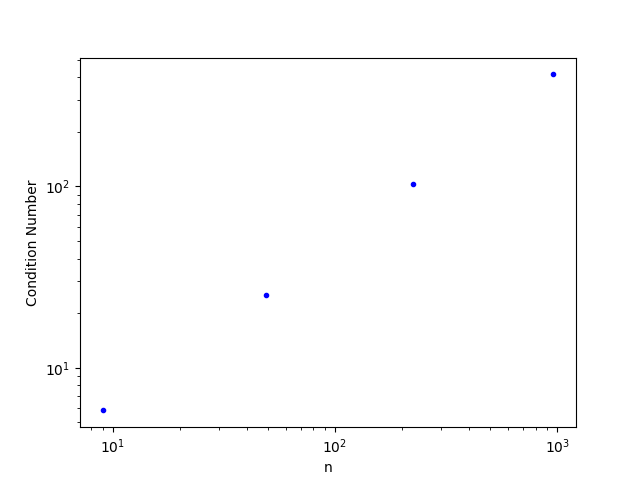
\includegraphics[width=1\textwidth]{hwch7_figure_1}
	\label{5c1}
	\centering
\end{figure}

\begin{figure}[H]
	\caption{Jacobi Method Performance $N=31, n=31^2$}
	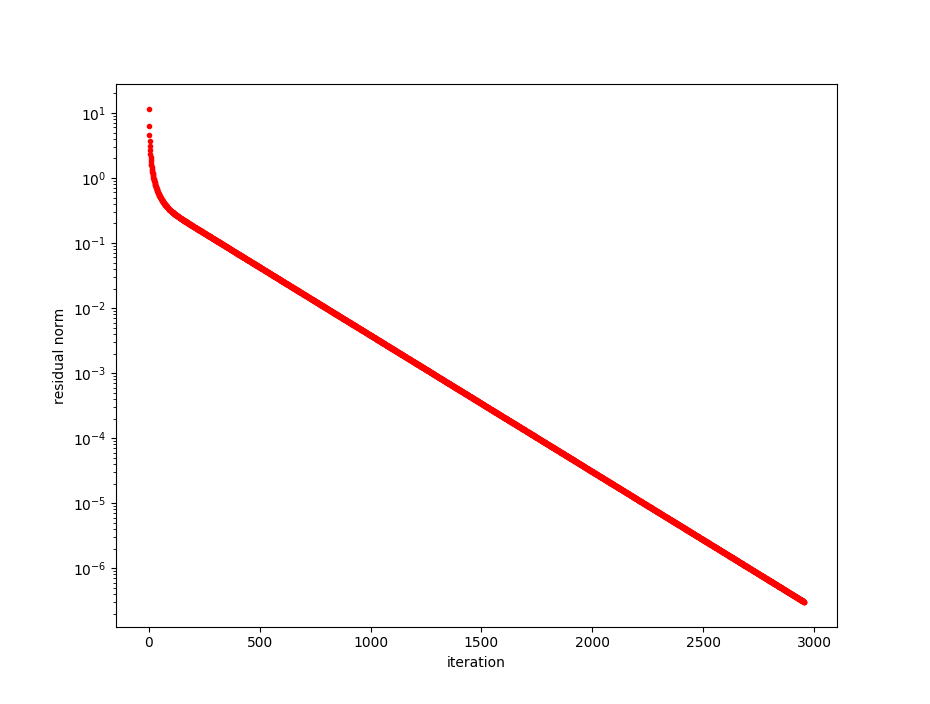
\includegraphics[width=1\textwidth]{hwch7_figure_2}
	\label{5c2}
	\centering
\end{figure}

As expected the condition number scales linearly with $n$ and it takes roughly a constant number of iterations to reduce the norm of the residual by a factor. From the table it seems that the number of iterations required scales linearly with $n$. 

\bigbreak
%%%%%%%%%%%%%%%%%%%%%%%%%%%%%%%%%%%%%%%%%%%%%%%%%%%%%%%%%%%%%%%%%%%%%%%%%%%%%%%%%%%%%%%%%%%%%%%%%%%%

\problem{9 (a)} Using the iteration scheme $x_{k+1} = x_k + \alpha(b-Ax_k)$ the splitting associated would be $A= M-N$ where $M^{-1} = \alpha I$. Then $M = \frac{1}{\alpha}I$ and
\begin{align*}
	T & = I - M^{-1}A \\
	& = I - \alpha I A \\
	& = I - \alpha A
\end{align*}

\bigbreak
%%%%%%%%%%%%%%%%%%%%%%%%%%%%%%%%%%%%%%%%%%%%%%%%%%%%%%%%%%%%%%%%%%%%%%%%%%%%%%%%%%%%%%%%%%%%%%%%%%%%

\problem{9 (b)} We have a theorem that says that a Stationary Method converges if and only if the spectral radius is less than one. Suppose that $A$ is SPD with eigenvalues $\lambda_1 > \lambda_2 > ... > \lambda_n > 0$. Then $T$ is symmetric. Suppose that $x_k$ is an eigenvector corresponding to the eigenvalue $\lambda_k$. Then
\begin{align*}
	Tx_k & = Ix_k - \alpha Ax_k \\
	& = x_k - \lambda_k \alpha x_k \\
	& = \left(1- \lambda_k \alpha \right)x_k
\end{align*}
Thus each eigenvector of $A$ is also an eigenvector of $T$ corresponding to an eigenvalue of $\left( 1- \lambda_k \alpha \right)$. Since $T$ is symmetric, $\rho(T) = \max\limits_k \{ \left\vert 1 - \lambda_k \alpha \right \vert \}$. In order for the method to converge, we require that this value be less than 1. \bigbreak

Suppose that $\alpha < 0$. Then we get that 
$$
- \lambda_1 \alpha > - \lambda_2 \alpha > ... > - \lambda_n \alpha > 0
$$
$$
1 - \lambda_1 \alpha > 1 - \lambda_2 \alpha > ... > 1 - \lambda_n \alpha > 1
$$
and our iterations fail to converge.
Suppose that $\alpha > 0$. Then
$$
1 - \lambda_1 \alpha < 1 - \lambda_2 \alpha < ... > 1 - \lambda_n \alpha < 1
$$
As long as $-1 < 1 - \lambda_1 \alpha $ this will converge. Solving for $\alpha$ we get our final result: \bigbreak

The iteration $x_{k+1} = x_k + \alpha(b-Ax_k)$ will converge if and only if $\frac{2}{\lambda_1} < \alpha$ where $\lambda_1$ is the largest eigenvalue of the SPD matrix $A$. \bigbreak

To maximize the rate of convergence we need to minimize the spectral radius. This is made simpler by noting that 
$$
\rho(T) = \max \left\{  \left\vert 1- \lambda_1\alpha \right\vert, \left\vert 1 - \lambda_2\alpha\right\vert \right \}
$$
since the eigenvalues are all between these two. Since $1-\lambda_1\alpha < 1 - \lambda_n\alpha$ we really only need to consider
$$
\rho(T) = \max \left\{  \lambda_1\alpha - 1 , 1 - \lambda_n\alpha \right \}
$$
In addition, since $\lambda_1\alpha - 1$ is increasing with $\alpha$ and $1 - \lambda_n\alpha$ is decreasing with $\alpha$, the $\rho(T)$ will reach a minimum at the intersection point. That is that the value of $\alpha$ that minimizes $\rho(T)$ satisfies
\begin{align*}
	\lambda_1\alpha - 1 & = 1 - \lambda_n\alpha \\
	(\lambda_1 + \lambda_n )\alpha & = 2 \\
	\alpha & = \frac{2}{\lambda_1 + \lambda_2}
\end{align*}
We can find the spectral radius in this case by
\begin{align*}
	\rho(T) & = lambda_1\alpha - 1 \\
	\rho(T) & = 1 - \lambda_n\alpha \\
	2 \rho(T) & = \alpha(\lambda_1 - \lambda_n) \\
	2 \rho(T) & = 2 \frac{\lambda_1 - \lambda_n}{\lambda_1 + \lambda_n} \\
	\rho(T) & = \frac{\kappa(A) - 1}{\kappa(A)+1}
\end{align*}
As $\kappa(A)$ gets large $\rho(T)$ approaches $1$ and converges slowly. 

\bigbreak
%%%%%%%%%%%%%%%%%%%%%%%%%%%%%%%%%%%%%%%%%%%%%%%%%%%%%%%%%%%%%%%%%%%%%%%%%%%%%%%%%%%%%%%%%%%%%%%%%%%%

\problem{9 (c)} The statement in the text is false. If $A$ is strictly diagonally dominant and $\alpha = 1$ the iterative scheme will only converge if $\lambda_1 > 2$

\bigbreak
%%%%%%%%%%%%%%%%%%%%%%%%%%%%%%%%%%%%%%%%%%%%%%%%%%%%%%%%%%%%%%%%%%%%%%%%%%%%%%%%%%%%%%%%%%%%%%%%%%%%

\problem{13 } The plot of the condition number of $A$ with $n$ is exactly the same as in problem 5 since the condition number does not depend on any method of solving the system. 

Since it was explicitly asked for in this problem, the code used to generate the results appears here instead of in an Appendix.

\begin{lstlisting}
def A_mult(x):
	n = len(x)
	N = int(np.sqrt(n))
	assert N**2 == n
	assert N>= 3
	r = np.zeros(n)
	r[0] = 4*x[0] - x[1] - x[N]
	for i in range(1, N):
		r[i] = -x[i-1] + 4*x[i] - x[i+1] - x[i+N]
	for i in range(N, n-N):
		r[i] = -x[i-N] - x[i-1] + 4*x[i] - x[i+1] - x[i+N]
	for i in range(n-N, n-1):
		r[i] = -x[i-N] - x[i-1] + 4*x[i] - x[i+1]
	r[-1] = -x[-1-N] - x[-2] + 4*x[-1]
	for i in range(N,n,N):
		r[i] += x[i-1]
	for i in range(N-1,n-1,N):
		r[i] += x[i+1]
	return r

def cg_solve(x, b, tol, max_iter=10**9):
	n = len(x)
	N = int(np.sqrt(n))
	assert N**2 == n
	assert N>= 3
	x_old = x
	r = residual(x_old, b)
	res_norms = [np.linalg.norm(r)]
	iterations = 1
	delta = np.dot(r, r)
	b_delta = np.dot(b,b)
	p = r
	while delta > b_delta * tol**2 and iterations < max_iter:
		s = A_mult(p)
		alpha = delta/np.dot(p,s)
		x_new = x_old + alpha*p
		r -= alpha * s
		res_norms.append(np.linalg.norm(r))
		delta_new = np.dot(r,r)
		p = r + delta_new/delta * p
		x_old, delta = x_new, delta_new
		iterations += 1
	cond = (1+np.cos(np.pi/(N+1)))/(1-np.cos(np.pi/(N+1)))
	return x_new, iterations, cond, res_norms
\end{lstlisting}

	\begin{center}
		\begin{tabular}{|c|c|c|c|c|c|}
			\hline
			$l$&$N$&$n$&iterations required&error at $(0.5,0.5)$&$\kappa(A)$\\ \hline
			2&3&9&21&3.339e-07&5.828e+00\\ \hline
			3&7&49&31&2.267e-07&2.527e+01\\ \hline
			4&15&225&54&3.442e-08&1.031e+02\\ \hline
			5&31&961&91&1.761e-07&4.143e+02\\ \hline
			6&63&3969&165&-2.676e-08&1.659e+03\\ \hline
		\end{tabular}
	\end{center}
		


\begin{figure}[H]
	\caption{Conjugate Gradient Performance $N=31, n=31^2$}
	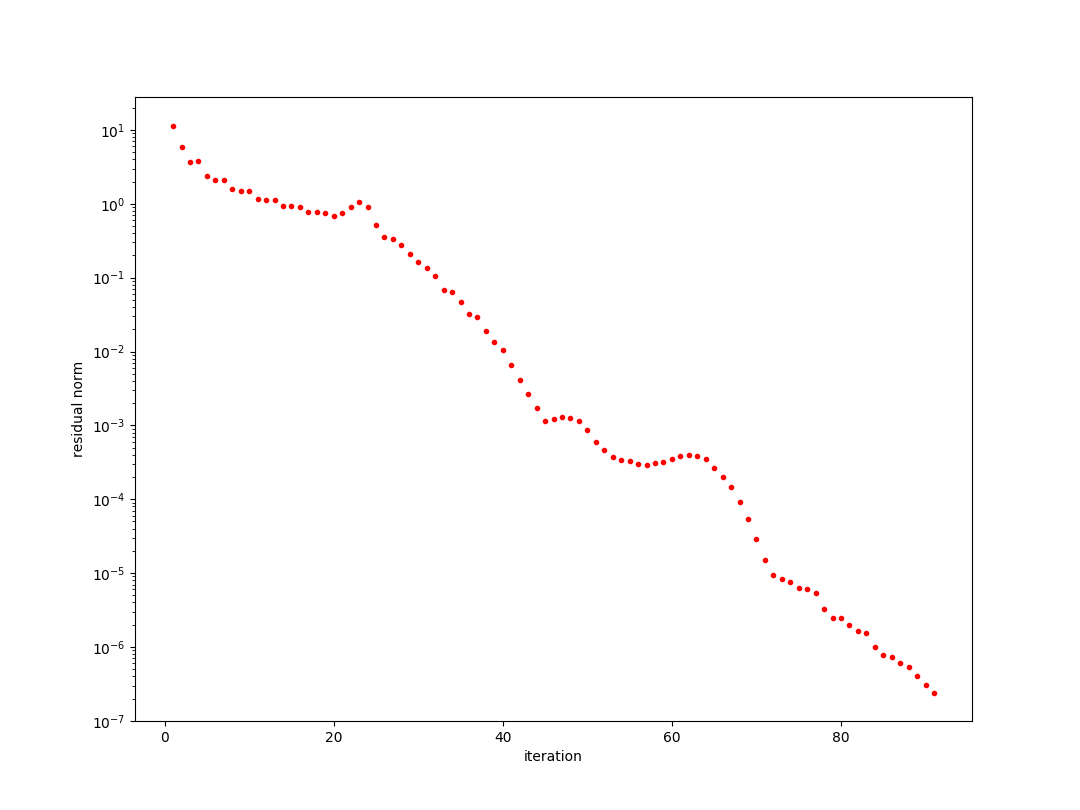
\includegraphics[width=1\textwidth]{hwch7_figure_3_cg_N31_2}
	\label{13c}
	\centering
\end{figure}

As $n$ gets larger the number of iterations drops dramatically and is always less than $n$. This is far better than the Jacobi Method. 

\bigbreak
%%%%%%%%%%%%%%%%%%%%%%%%%%%%%%%%%%%%%%%%%%%%%%%%%%%%%%%%%%%%%%%%%%%%%%%%%%%%%%%%%%%%%%%%%%%%%%%%%%%%

\problem{25 (a)} Applying finite differences to the Helmoholtz equation we get
\begin{align*}
	4u_{i,j} - u_{i+1,j} - u_{i-1,j} - u)_{i,j+1} - u_{i,j-1} - \omega^2 h^2 u_{i,j} & = b_{i,j} \\
	(4- (\omega h)^2)u_{i,j} - u_{i+1,j} - u_{i-1,j} - u_{i,j+1} - u_{i,j-1} & = b_{i,j}
\end{align*}
where $b_{i,j} = h^2g(ih,jh)$ as in the text. This leads to an $A$ matrix similar to example 7.1 except that it has $4-(\omega h)^2$ for each diagonal element entry instead of $4$ for each diagonal entry. \bigbreak

\bigbreak
%%%%%%%%%%%%%%%%%%%%%%%%%%%%%%%%%%%%%%%%%%%%%%%%%%%%%%%%%%%%%%%%%%%%%%%%%%%%%%%%%%%%%%%%%%%%%%%%%%%%

\problem{15 (b)} If we let $A^\prime$ represent the matrix from example 7.1 (the one with $4$ along the diagonal) then our matrix would be given by $A = A^\prime- I(\omega h)^2$. Suppose that $\lambda$ is an eigenvalue of $A$. Then
\begin{align*}
	0 & = A - \lambda I \\
	& = A - (\lambda + (\omega h)^2 - (\omega h)^2)I \\
	& = A - \lambda I - (\omega h)^2I + (\omega h)^2I \\
	& = (A + (\omega h)^2I) - (\lambda + (\omega h)^2)I \\
	& = A^\prime - (\lambda + (\omega h)^2)I
\end{align*}
Thus concluding that $\lambda + (\omega h)^2$ is an eigenvalue of $A^\prime$. This tells us that all of the eigenvalues of $A$ are given by
$$
\lambda_{l,m} = 4 - 2(\cos(l \pi h) + \cos(m \pi h)) - (\omega h)^2, 1\leq l,m \leq N
$$

In order for $A$ to be positive definite, we need need for all of the eigenvalues to remain positive. Thus the $\omega_c^2h^2$ we seek is simply the smallest eigenvalue of $A^\prime$. Thus
\begin{align*}
	\omega_c^2h^2 & = 4 - 4 \cos\left(\frac{1 }{N+1}\pi \right) \\
	\omega_c & = 2h \sqrt{1- \cos\left(\frac{1 }{N+1}\pi \right)}
\end{align*}

\bigbreak
%%%%%%%%%%%%%%%%%%%%%%%%%%%%%%%%%%%%%%%%%%%%%%%%%%%%%%%%%%%%%%%%%%%%%%%%%%%%%%%%%%%%%%%%%%%%%%%%%%%%

\problem{15 (c)} Code for this part was taken largely from the author's code for example 7.7, though some modifications were made. This was tested using the dampened Jacobi method for both relaxation steps, and again using Minres for both relaxation steps. The results were identical. Both methods were effective at reducing oscillations in the residual allowing the multigrid method to quickly reduce the smoothed residual. The number of multigrid cycles required did not change significantly with $N$.

\begin{figure}[H]
	\caption{Multigrid method applied to the Helmoholtz equation with $\omega = 1$}
	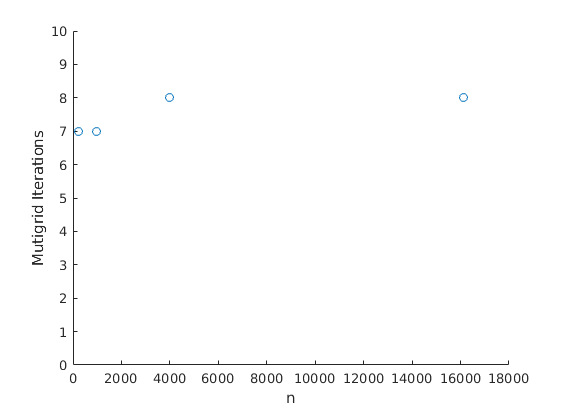
\includegraphics[width=.75\textwidth]{hwch7_figure_4_multigrid_w1_jacobi}
	\label{multigrid}
	\centering
\end{figure}

On checking the norms of the residuals we can see that they are way below the set tolerance further emphasizing the impressive convergence speed of multigrid methods. In the table below, $l$ is given along with the norm of the residual where $N = 2^l-1$.

	\begin{center}
		\begin{tabular}{|c|c|c|c|}
			\hline
			$l$ & $N$ & $n$ & $\norm{r}$\\ \hline
			4& 15 & 225 & 9.086750e-09\\ \hline
			5& 31 & 961 & 2.824305e-08\\ \hline
			6& 63 & 3969 & 4.440823e-09\\ \hline
			7& 127 & 16129 & 3.003766e-09\\ \hline
		\end{tabular}
	\end{center}



\bigbreak

{\hspace{-4 ex} \huge \textbf{Appendix - Code listings}}\bigbreak

\large{Problem 25(c) code:}
\begin{lstlisting}[language=MATLAB]
clear all
close all
% This code is a modified version of the code used in example 7.7
% https://www.mathworks.com/support/books/book69732.html

l = 7;
ns = zeros(4,1);
iterations = zeros(4,1);
for i=1:4
l = i+3;
N = 2^l - 1;

%N = 2^7 -1;
tol = 1.e-6;  % should actually depend on N but never mind.


w = 1;
h = 1/(N+1);
n = N^2;
ns(i,1) = n;
A = delsq(numgrid('S',N+2)) - diag(ones(n,1).*(w*h)^2);
%n = size(A,1);
b = ones(n,1)*h^2;

% Solve using multigrid
xmg = zeros(n,1); bb = norm(b);
flevel = log2(N+1);
for itermg = 1:30
	[xmg,res] = poismg(A,b,xmg,flevel);
	if res/bb < tol
		break;
	end
end
%[xmg, ~, ~, itermg] = minres(A,b,tol,1000);
iterations(i,1) = itermg;
fprintf("%i: %e\n", l, norm(A*xmg - b));
end

hold on
plot(ns, iterations,'o');
xlabel("n");
ylabel("Mutigrid Iterations");
ylim([0,10]);
hold off
\end{lstlisting}

\large{Code for the poismg function}
\begin{lstlisting}[language=MATLAB]
% This code is a modified version of the code used in example 7.7
% https://www.mathworks.com/support/books/book69732.html


function [x,res] = poismg(A,b,x,level,tol)
%
% function [x,res] = poismg(A,b,x,level)
%
% multigrid V-cycle to solve simplest Poisson on a square
% The uniform grid is N by N, N = 2^l-1 some l > 2,
% b is the right hand side; homogeneous Dirichlet;
% A has been created by   A = delsq(numgrid('S',N+2));

coarsest = 3;              % coarsest grid
nu1 = 2;                   % relaxations before coarsening grid
nu2 = 2;                   % relaxations after return to finer level
omeg = .8;                 % relaxation damping parameter

if level == coarsest
x = A\b;               % solve exactly on coarsest level
r = b - A*x;

else % begin multigrid cycle

% relax using damped Jacobi
Dv = diag(A);         % diagonal part of A as vector
for i=1:nu1
	r = b - A*x;
	x = x + omeg*r./Dv;
end
% relax using minres
%x = minres(A,b,10,tol,nu1);

% restrict residual from r to rc on coarser grid
r = b - A*x; 
N = sqrt(length(b));
r = reshape(r,N,N);
Nc = (N+1)/2 - 1; nc = Nc^2;    % coarser grid dimensions
Ac = delsq(numgrid('S',Nc+2));  % coarser grid operator
rc = r(2:2:N-1,2:2:N-1) + .5*(r(3:2:N,2:2:N-1)+r(1:2:N-2,2:2:N-1) +...
	r(2:2:N-1,3:2:N)+r(2:2:N-1,1:2:N-2)) + .25*(r(3:2:N,3:2:N)+...
	r(3:2:N,1:2:N-2)+r(1:2:N-2,3:2:N)+r(1:2:N-2,1:2:N-2));
rc = reshape(rc,nc,1);

% descend level. Use V-cycle
vc = zeros(size(rc));            % initialize correction to 0
[vc,r] = poismg(Ac,rc,vc,level-1); % samesame on coarser grid

% prolongate correction from vc to v on finer grid
v = zeros(N,N);
vc = reshape(vc,Nc,Nc);
v(2:2:N-1,2:2:N-1) = vc;
vz = [zeros(1,N);v;zeros(1,N)];   % embed v with a ring of 0s
vz = [zeros(N+2,1),vz,zeros(N+2,1)];
v(1:2:N,2:2:N-1) = .5*(vz(1:2:N,3:2:N)+vz(3:2:N+2,3:2:N));
v(2:2:N-1,1:2:N) = .5*(vz(3:2:N,1:2:N)+vz(3:2:N,3:2:N+2));
%v(3:2:N-2,3:2:N-2) = .25*(v(2:2:N-3,2:2:N-3)+v(2:2:N-3,4:2:N-1)+...
%    v(4:2:N-1,4:2:N-1)+v(4:2:N-1,2:2:N-3));
v(1:2:N,1:2:N) = .25*(vz(1:2:N,1:2:N)+vz(1:2:N,3:2:N+2)+...
	vz(3:2:N+2,3:2:N+2)+vz(3:2:N+2,1:2:N));

% add to current solution
n = N^2;
x = x + reshape(v,n,1);

% relax using damped Jacobi
for i=1:nu2
	r = b - A*x;
	x = x + omeg*r./Dv;
end
% relax using minres
%x = minres(A,b,10,tol,nu2);

end
res = norm(b - A*x);
\end{lstlisting}

\end{document}
